% このフォルダは修士・博士輪講のハンドアウトのテンプレート用です.適当に改変して使ってください.
% 現在Overleaf上でコンパイル出来ることは確認しています (2020/06/10)
% This folder is for a template file for master/doctor Rinko. Feel free to modify it.
% This file can be compiled on Overleaf-v2.
\documentclass[xelatex,a4j,10pt,twocolumn]{article}
\usepackage[utf8]{inputenc}
\usepackage[whole]{bxcjkjatype}

\usepackage{balance}
\setlength{\textwidth}{180mm}
\setlength{\textheight}{250mm}
\setlength{\oddsidemargin}{-10mm}
\setlength{\evensidemargin}{-10mm}
\setlength{\topmargin}{-15mm}

\usepackage[dvipdfmx]{color}
\usepackage[dvipdfmx]{graphicx}
\usepackage{framed}
\usepackage{nidanfloat}


% change fontsize / margin in references
\makeatletter
\renewenvironment{thebibliography}[1]
{\section*{\refname\@mkboth{\refname}{\refname}}%
	\list{\@biblabel{\@arabic\c@enumiv}}%
	{\settowidth\labelwidth{\@biblabel{#1}}%
		\leftmargin\labelwidth
		\advance\leftmargin\labelsep
		\setlength\itemsep{0ex} % interval between lines
		\setlength\baselineskip{10pt} % fontsize
		\@openbib@code
		\usecounter{enumiv}%
		\let\p@enumiv\@empty
		\renewcommand\theenumiv{\@arabic\c@enumiv}}%
	\sloppy
	\clubpenalty4000
	\@clubpenalty\clubpenalty
	\widowpenalty4000%
	\sfcode`\.\@m}
{\def\@noitemerr
	{\@latex@warning{Empty `thebibliography' environment}}%
	\endlist}
\makeatother

% change the top/bottom margin (0.6 / 0.4 default)
% \makeatletter
% \renewcommand{\section}{%
% 	\@startsection{section}{1}{\z@}%
% 	{0.6\Cvs}{0.4\Cvs}%
% 	{\normalfont\large\headfont\raggedright}}
% \makeatother

\begin{document}

%------------------------------------------------------------ title
\twocolumn[
\begin{framed}
	大学院輪講資料 \hfill2022年11月11日% year, month, and day
    \begin{center}
        % title in Japanese/English
		\textbf{
			{\Large 画像の美的属性評価に関する研究動向} \\
			{\Large A Survey on Aesthetic Attributes Assessment of Images}
		}
	\end{center}
	山崎研究室 \hfill 電子情報学専攻 修士課程1年 48-226444 付琛  % student ID and name
\end{framed}
\vspace{20pt}
]

\section*{Abstract}
\label{sec:abstract}
Image aesthetic quality assessment has been a hot topic in the past decade. Recently, review-type textual evaluations have been used to describe the general aesthetic impression of images. For an input image, the image aesthetic quality assessment model can generate a text describing the aesthetic properties of the image. On the one hand, this review-type text evaluation can intuitively reflect people's true feelings about images. On the other hand, with the advent of the information age, the image aesthetic quality assessment model model can guide us to optimize a variety of images, such as advertising images, clothing images and other images with commercial value.

In this survey, I introduce some basic models and implementation methods of image aesthetic attribute evaluation. The evaluation of the aesthetic properties of images is often based on Image captioning work. I introduce the basic principles of Image captioning work and its development in recent years. On this basis, the image quality aesthetic evaluation methods such as AMAN will also be introduced in this survey.


\section{Introduction}
\label{sec:introduction}
Image aesthetic quality assessment is to evaluate images for aesthetic aspects. In recent years, image aesthetic quality assessment has attracted a lot of interest in the commercial fields of computer vision, computational aesthetics, psychology, neuroscience, and advertising. Image aesthetic quality assessment attempts to classify input images into two categories: high aesthetic quality images and low aesthetic quality images. In order to enrich the form of image aesthetic quality assessment, textual and numerical scores. are introduced into the image aesthetic quality assessment model.

Image Captioning work is the basis for image aesthetic quality assessment. The main task of Image Captioning work is to generate corresponding text descriptions for input images. It uses CNN-LSTM as its basic architecture and has achieved great success in text generation. In recent years, various architectures such as attention mechanism and transformer have been introduced into image captioning work. This greatly enriches the text content it generates.

Composition mainly considers the stability of the whole picture. The so-called stability is a visual habit and aesthetic concept naturally formed by human beings in long-term observation. In life, only the plastic arts that conform to this aesthetic concept can produce beauty; and images that violate this principle often do not look beautiful. Stable does not mean that the elements in the image are evenly distributed, but that there is a logical proportional relationship between all the elements in the image. Symmetric distributions are typical of this view.

Color is an important aesthetic attribute in image evaluation. For the aesthetic feeling that an image brings to people, image aesthetic quality evaluation is often considered from the three characteristics of hue, lightness and saturation.

The focal point of an image is an important part of the image. Without a fixed point of interest, the image will appear cluttered and fail to capture the viewer's attention; on the other hand, an image with a strong point of interest will immediately reveal the main content of the image to the viewer. Bringing out the focal point of the image is especially important for commercially valuable images such as advertising images.

In order to get the evaluation of images on different aesthetic attributes, I will introduce the aesthetic multi-attribute evaluation network. The network structure is based on image captioning work with attention mechanism, trying to give text evaluation and numerical score for different aesthetic attributes.

\section{Image captioning}
Image captioning\cite{9cap,10cap,11cap} means automatically generating a caption for an image. As a recently emerged research area, it is attracting more and more attention. To achieve the goal of image captioning, semantic information of images needs to be captured and expressed in natural languages. Connecting both research communities of computer vision and natural language processing, image captioning is a quite challenging task. Various approaches have been proposed to solve this problem.Based on the technique adopted, we can classify image captioning approaches into different categories.

Representative methods in each category are summarized, and their strengths and limitations are talked about. We first discuss methods used in early work which are mainly retrieval and template based. And in this survey, we focus our main attention on neural network based methods, which give state of the art results. Neural network based methods are further divided into subcategories based on the specific framework they use.
\subsection{CNN + LSTM}

\begin{figure}[h]
	\leftmargin
    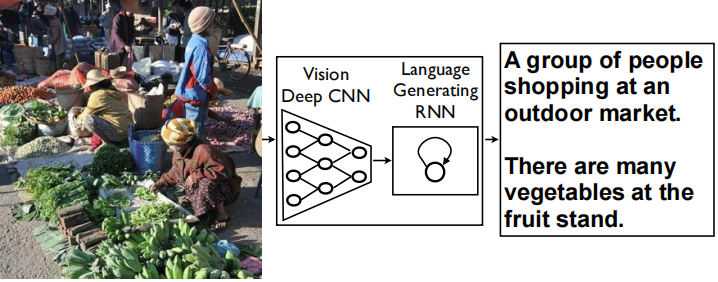
\includegraphics[width=0.5\textwidth]{NIC.png}
 	\caption{NIC model}
 	\label{fig:NIC MODEL}
\end{figure}

The CNN+LSTM in the NIC model\cite{DBLP} of the most classic deep learning models in the field of image captioning. In the image description work, we mainly deal with two different modalities of information: one is the image, and the other is the description text. Tasks such as object detection, image segmentation, and image recognition only involve the processing of images, while in natural language processing, text generation, automatic summarization, and pre-training models only involve textual information. On this basis, the NIC model effectively realizes the interaction between image and text information.

\begin{figure}[h]
	\centering
    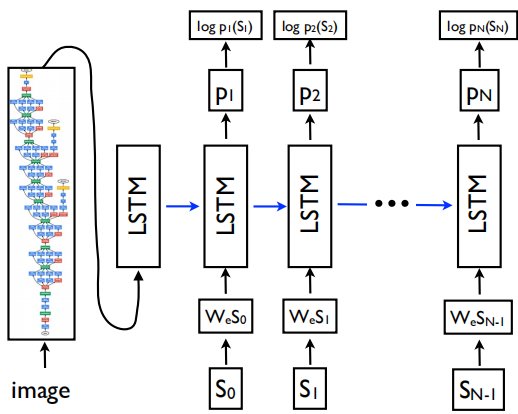
\includegraphics[width=0.5\textwidth]{NIC1.png}
 	\caption{NIC network}
 	\label{fig:NIC MODEL}
\end{figure}

From the network of NIC model,the input image is subjected to CNN to extract image features. The feature vector is averaged in the height and width dimensions, so that its physical meaning represents the global information features of the image, and then the global information features are sent to the LSTM.The LSTM model \cite{8LSTM}is trained to predict each word of the sentence after it has seen the image as well as all preceding words as defined by  p(S\_t|I,S\_0,...S\_t-1).

In more details,if we denote by \textit{I} the input image and by S = (S\_0,...,S\_N),which is a true sentence describing this image,the unrolling procedure reads:

\begin{equation}
x_0 = CNN(I)
\end{equation}

\begin{equation}
x_t = W_t*S_t    
\end{equation}

\begin{equation}
p(t)=LSTM(x_t)
\end{equation}
where this model represent each as a one-hot vector S\_t of dimension equal to the size of the dictionary.Note that we denote by S\_0 a special start word and by S\_N a special stop word which designates the start and end of the sentence.

\subsection{Attention Mechanism}
Inspired by the work in machine translation and object detection,attention based model has been introduced to solve the problem of describing the content of images.Here in this survey,I'd like to introduce 2 papers here.
\subsubsection{Neural Image Caption Generation with Visual Attention}
The paper\cite{2DBLP} about neural image caption generation with visual attention describe how to train this model in a deterministic manner using standard backpropagation techniques and stochastically by maximizing a variational lower bound.
They achieve this model mainly based on the framework of Encoder-Decoder Network.In this part,the paper used the CNN as encoder and LSTM as decoder.

Stochastic attention and deterministic attention was introduced into this model.In the next paragraphs there are more details about these two attention mechanisms.

Stochastic attention:the paper represent the location variable \textit{St} as where the model decides to focus attention when generating the t-th word. St is an indicator one-hot variable which is set to 1 if the i-th location (out of L) is the one used to extract visual features. By treating the attention locations as intermediate latent variables, we can assign a multinoulli distribution parametrized by a, and view z as a random variable: 
\begin{equation}
    p(s_t = 1)= \alpha_t
\end{equation}
\begin{equation}
    z_t = \sum s_t\times\alpha_i
\end{equation}

Then the paper define a new objective function L\_s that is a variational lower bound on the marginal log-likelihood log p(y|a)of observing the sequence of words y given image features
similar to work in generative deep generative modeling the learning algorithm for the parameters W of the models can be derived by directly optimizing and futher  reduce the variance to get the final learning rule for the model.There are two hyper-parameters set by cross validation.
\begin{equation}
    L_s = \sum p(s|a)logp(y|s,a)
        = log p(y|a)
\end{equation}

\begin{equation}
\begin{split}
    \frac{\partial L_S}{\partial W} = \frac{1}{N}\sum\frac{\partial log p(y|s^n,a)}{\partial W}+\lambda_r(log p (y|s^n,a)-b) \\
    + \lambda_e\frac{\partial H[s^-n]}{\partial W}    
\end{split}
\end{equation}

Deterministic attention: it can also be understood as approximately optimizing the marginal likelihood under the attention location random variable s. The hidden activation of LSTM h is a linear projection of the stochastic context vector zˆt followed by tanhnon-linearity. To the first-order Taylor approximation, the expected value E is equivalent to computing h using a single forward computation with the expected context vector E.
\begin{figure*}[t]
	\centering
    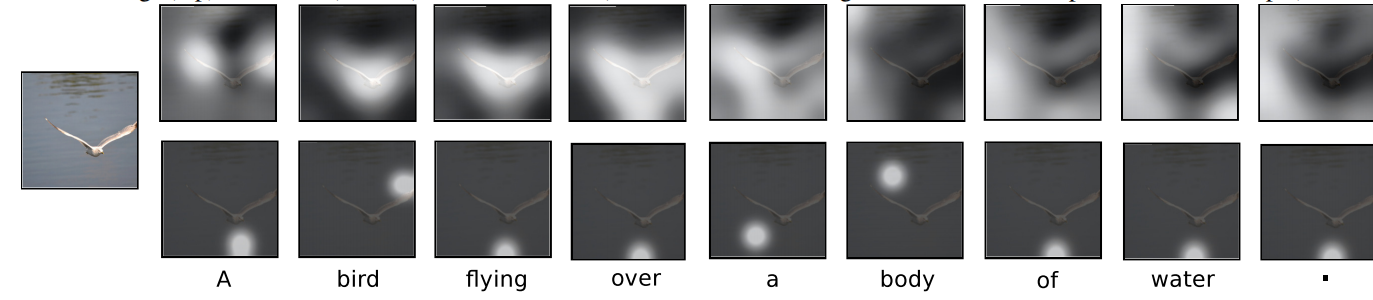
\includegraphics[width=1\textwidth]{3atten.png}
 	\caption{Result of Neural Image Caption Generation with Visual Attention. Visualization of the attention for each generated word.}
 	\label{fig:3atten}
\end{figure*}

\subsubsection{Bottom-Up and Top-Down Attention for Image Captioning}
\begin{figure}[h]
	\centering
    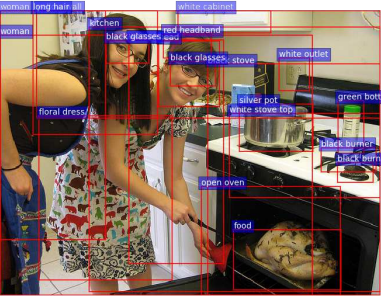
\includegraphics[width=0.5\textwidth]{4.png}
 	\caption{Result Example output from our Faster R-CNN bottom-up attention model.}
 	\label{fig:4}
\end{figure}
Bottom-Up and Top-Down Attention for Image Captioning \cite{3BUTD}is another model which enables attention to be calculated at the level of objects and other salient image regions.Within this approach,the bottom-up mechanism(mainly based on Faster R-CNN)proposes image regions,each with an associated feature vector,while top-down mechanism determines feature weightings.

The definition of spatial image features V is generic.However, in this work they define spatial regions in terms of bounding boxes and implement bottom-up attention using Faster R-CNN instead of CNN.In this paper,faster R-CNN can detect objects in two stages. The first stage, which can be described as a Region Proposal Network (RPN), predicts object proposals. A small network is slid over features at an intermediate level of a CNN. At each spatial location the network predicts a class-agnostic objectness score and a bounding box refinement for anchor boxes of multiple scales and aspect ratios. Using greedy non-maximum suppression with an intersection-over-union (IoU) threshold, the top box proposals are selected as input to the second stage. In the second stage, region of interest (RoI) pooling is used to extract a small feature map for each box proposal. These feature maps are then batched together as input to the final layers of the CNN. The final output of the model consists of a softmax distribution over class labels and class-specific bounding box refinements for each box proposal.

\begin{figure}[h]
	\centering
    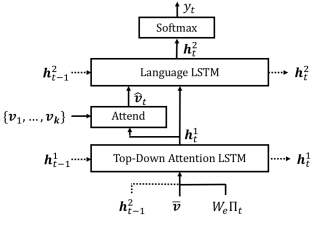
\includegraphics[width=0.5\textwidth]{5.png}
 	\caption{Overview of the proposed captioning model. Two LSTM
layers are used to selectively attend to spatial image features}
 	\label{fig:5}
\end{figure}
In this paper,for given image features V,the captioning model uses a 'soft' top-down attention mechanism to weight each feature during caption generation,with the partial output sequence as context.At a high level the captioning models is composed of two LSTM layers using a standard implementation.where \textit{X} is the LSTM input vector and h is the LSTM output vector. Here they have neglected the propagation of memory cells for notational convenience. Finally they describe the formulation of the LSTM input vector \textit{X} and the output vector \textit{h} for each layer of the model.

\begin{equation}
    h_t = LSTM(X_t,h_t_-_1)
\end{equation}







\subsection{Transformer + LSTM}
As this survey mentioned above, the architecture of CNN+LSTM has made outstanding contributions in the field of image captioning. Next I will continue to introduce two other papers based on the Tensor+LSTM framework.
\subsubsection{Attention on Attention for Image Captioning}
\begin{figure}[h]
	\centering
    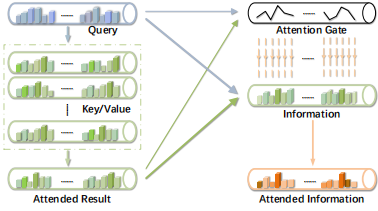
\includegraphics[width=0.5\textwidth]{6.png}
 	\caption{Attention on Attention (AoA). AoA generates an
information vector and an attention gate using the attention result and the attention query, and adds another attention by applying the gate to the information and obtains the
attended information}
 	\label{fig:6}
\end{figure}

In this paper\cite{4}, they propose an “Attention on Attention” (AoA) module, which extends the conventional attention mechanisms to determine the relevance between attention results
and queries. AoA first generates an “information vector” and an “attention gate” using the attention result and the current context, then adds another attention by applying element-wise multiplication to them and finally obtains the “attended information”, the expected useful knowledge.This paper also apply AoA to both the encoder and the decoder of image captioning model, which is named as AoA Network(AoANet).

An attention module function(Q, K, V ) operates on some queries, keys and values and generates some weighted average vectors (denoted by Q, K, V and Vˆ respectively). It first measures the similarities between Q and K and then uses the similarity scores to compute weighted average vectors over V,which can be formulated as:

\begin{equation}
    a_i_,_j = f_s_i_m(q_i,k_j)=\frac{e^a_i^,^j}{\sume^a_i^,^j}
\end{equation}



\begin{equation}
    v_i = \sum a_i_,_j v_j
\end{equation}
The attention module outputs a weighted average for each query, no matter whether or how Q and K/V are related. Even when there is no relevant vectors, the attention
module still generates a weighted average vector, which can be irrelevant or even misleading information.
Thus this paper propose the AoA module to measure the relevance between the attention result
and the query. The AoA module generates an “information
vector” i and an “attention gate” \textit{g} via two separate linear transformations, which are both conditioned on the attention result and the current context  \textit{q}:
\begin{equation}
    i = W_q q +W_v V +b^i 
\end{equation}

\begin{equation}
    g=\sigma( W_q q +W_v V +b^G)
\end{equation}
Then AoA adds another attention by applying the attention gate to the information vector using element-wise multiplication and obtains the attended information \textit{i}:
\begin{equation}
   i = g * i 
\end{equation}

\subsubsection{Dual-Level Collaborative Transformer for Image Captioning}
\begin{figure}[h]
	\centering
    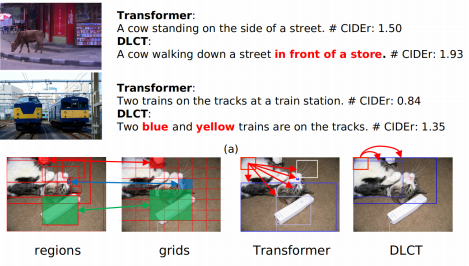
\includegraphics[width=0.5\textwidth]{7.png}    
 	\caption{Dual-Level Collaborative Transformer for Image Captioning}
 	\label{fig:7}
\end{figure}
Dual-Level Collaborative Transformer (DLCT) network\cite{5DLCT} is to realize the complementary advantages of the two features.In DLCT, there is a novel Dual-way Self Attenion (DWSA) to mine their intrinsic properties,where a Comprehensive Relation Attention component is also introduced to embed the geometric information. In addition,this paper propose a Locality-Constrained Cross Attention module to address the semantic noises caused by the direct fusion of these two features, where a geometric alignment graph is constructed to accurately align and reinforce region and grid features.

Dual-Way Self Attention : In general, visual features are
extracted by locally-connected convolutions, which make these features isolated and relation-agnostic. It is believed that Transformer Encoder contributes significantly to the performance
of image captioning, because it can model relationships between the inputs to enrich visual features by self-attention.
To better model intra-level relationships of two kinds of features, we devise a Dual-Way Self Attention (DWSA) which
consists of two independent self-attention modules.
Specifically, the hidden states of regions \textit{H}:
\begin{equation}
    C^(^l^) _r = MHCRA(H^(^l^) _r,H^(^l^) _r,H^(^l^) _r,RPE,RPE,\omega_r_r)
\end{equation}

\begin{equation}
    C^(^l^) _g = MHCRA(H^(^l^) _g,H^(^l^) _g,H^(^l^) _g,RPE,RPE,\omega_g_g)
\end{equation}
Then this paper adopt two independent position-wise feedward networks FFN for each type of visual features:
\begin{equation}
    C^(^l^) _r = FFN_r( C^(^l^) _r)
\end{equation}

\begin{equation}
    C^(^l^) _g = FFN_r( C^(^l^) _g)
\end{equation}
After that, the relation-aware representations are fed into the
next module.

Locality-Constrained Cross:In this paper,attention they propose Locality-Constrained Cross Attention (LCCA) to model complex interactions between regions and grids for inter-level fusion. To avoid introducing semantic noises, this paper first create a geometric alignment graph G = (V, E). All region and grid features are represented as independent nodes to form a visual node set V . For edge set E, a grid node is connected to a region node if and only if their bounding boxes have intersections. Following the above rules,this paper get an undirected graph.Based on the geometric alignment graph, this paper apply LCCA to identify attention across two different kinds of visual feature fields: the source field and the target field. In LCCA,the source field serves as queries and the target field serves as keys and values. LCCA aims at reinforcing representation of the source field by embedding information of the target field into the source field. And this paper also integrate the absolute and relative location information to get the weight matrix W and normalize it.

With these two attention network,this region can make alignment with one or more grids while a
grid can align with zero or more regions. There might exist a grid that aligns with no region. So a self-connected edge for each node in the geometric alignment graph will also do some help. Besides, self-connected edges give the attention module an extra choice of not attending to any other features. In the l-th layer, the attention module is followed by two independent \textit{FFN} like in DWSA:

\begin{equation}
    H^(^l^+^1^) _r = FFN_r ^l( M^(^l^) _r)
\end{equation}

\begin{equation}
    H^(^l^+^1^) _g = FFN_g ^l( M^(^l^) _g)
\end{equation}

\begin{figure*}[t]
	\centering
    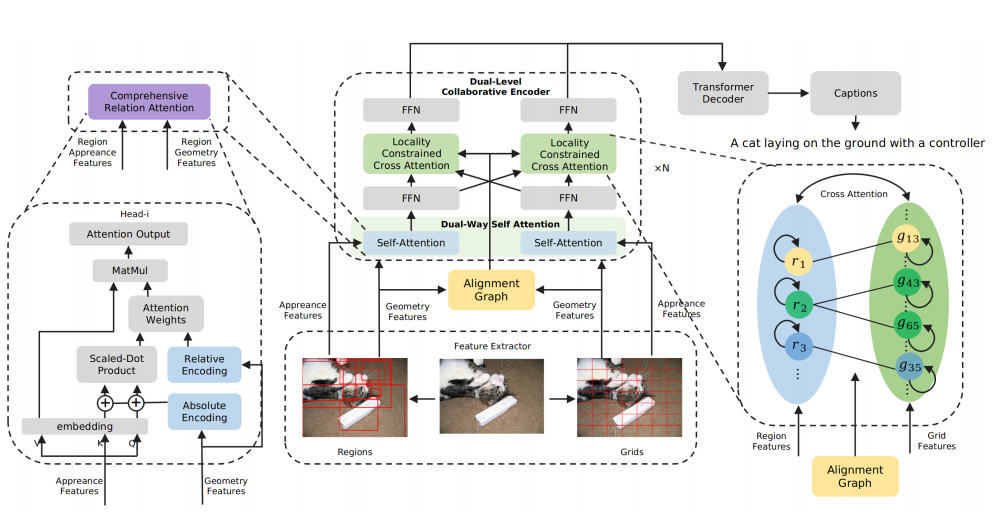
\includegraphics[width=1\textwidth]{8.png}    
 	\caption{Overview of the proposed Dual-Level Collaborative Transformer architecture.The Dual-Way Self Attention is applied tomine the intrinsic properties of two kinds of features, followed by the Locality-Constrained Cross Attention (LCCA) which enables the interaction between regions and grids. With the geometric alignment graph, LCCA can eliminate semantic noises
and achieve inter-level fusion effectively.}
 	\label{fig:8}
\end{figure*}



Image aesthetic quality assessment has been a relatively hot topic during the last decade. Most recently, comments type assessment has been proposed to describe the general aesthetic impression of an image using text. In these following papers,I'll introduce Aesthetic Attributes Assessment of Images, which means the aesthetic attributes captioning. This is a new formula of image aesthetic assessment, which predicts aesthetic attributes captions together with the aesthetic score of each attribute.

\section{Aesthetic Multi-Attribute Network (AMAN)}



Image Aesthetic Quality Assessment (IAQA) \cite{6AMAN,13}is to give an assessment of images on the aspect of aesthetics. In the last decades, IAQA has gained a great interest in the community of computer vision,
computational aesthetics, psychology and neuroscience.Most literatures of IAQA are to classify images into 2 categories:high aesthetic quality (professional) and low aesthetic quality (amateur). The second popular assessment task is to give a continuously numerical score of aesthetics. Another numerical assessment task is to predict a score distribution of human rating on the aesthetic aspect of an image.

\begin{figure*}[t]
	\centering
    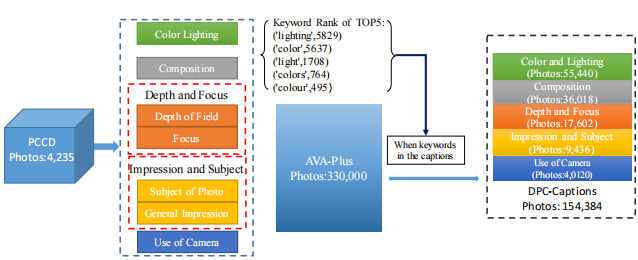
\includegraphics[width=1\textwidth]{9.png}    
 	\caption{The basic knowledge of datasets.Color Lighting, Composition, Depth of Field, Focus,General Impression and Use of Camera have become important properties for image aesthetic assessment work}
 	\label{fig:9}
\end{figure*}

\begin{figure*}[t]
	\centering
    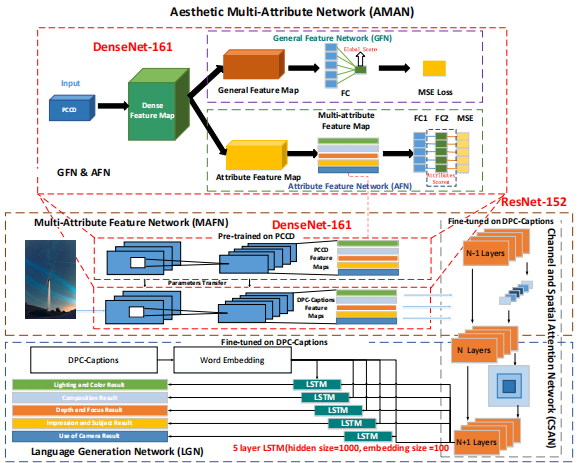
\includegraphics[width=1\textwidth]{10.png}    
 	\caption{Aesthetic Multi-Attribute Network (AMAN) contains Multi-Attribute Feature Network (MAFN), Channel and Spatial Attention Network (CSAN), and Language Generation Network (LGN).}
 	\label{fig:10}
\end{figure*}


\subsection{Datasets}
For a human artist, when shown a photo or a drawing, he/she will not just give a numerical score but always say a paragraph to describe many aesthetic attributes such as composition, lighting,color, focus of the image.In this paper,there are some datasets for Image Aesthetic Quality Assessment (IAQA) with name of Photo Critique Captioning Dataset (PCCD)\cite{7PDD} for the community. The PCCD contains 4,235 images and 29,645 comments. Each image is attached with comments and scores of 7 aesthetic attributes. However, they only output a sentence of assessment, which can not give a full review of aesthetic attributes. The value of PCCD is not fully explored. Besides, the size of PCCD is relatively small.

With the help of PCCD dataset, images of DPC-Captions are selected in this paper. The aesthetic attributes of PCCD dataset include Color Lighting, Composition, Depth of Field, Focus,General Impression and Use of Camera. For each aesthetic attribute,keywords of top 5 frequency are selected from the captions. This paper omit the adverbs, prepositions and conjunctions and combine words
with similar meaning such as color and colour, color and colors.

\subsection{Multi-Attribute Feature Network (MAFN)}

Multi-task learning is a common method widely used in training deep convolutional networks. Due to the diversity of the at￾tributes, multi-task learning can achieve multi-attribute assessment of aesthetics through parameter sharing. The aesthetic attributes assessment are relatively independent. However, the model training Channel and Spatial Attention Network (CSAN) process is similar. In PCCD, in addition to scores for each attribute, there is a global score for each image. Thus, the loss of MAFN is divided into two parts. One is the loss of each attribute (m attributes,in this paper m = 5). The other is the global loss. N represents the number of images in a batch. \textit{y} represents the output of the last fully connected layer of the network,which represents the true score.In this paper,they calculate global loss and single attribute loss. There are totally 6 loss layers in this model.
\begin{equation}
    Loss^A^t^t^r^i^b^u^t^e = Loss^G^l^o^b^a^l = \frac{1}{2N} \sum  ||y`-y^i||^2
\end{equation}
\begin{equation}
    Loss = \sum Loss^A^t^t^r^i^b^u^t^e + Loss^G^l^o^b^a^l 
\end{equation}
MAFN can extract different attribute feature maps of the image at the same time. Thus, the model is no longer limited to output comment of one sentence. The aesthetic characteristics of the image can be assessment from multiple attributes to better guide comprehensive assessment of images. The specific results obtained by the multi-task networks can also directly use the knowledge migrated to expand the attribute assessment of the DPC-Captions dataset,thus providing a broader aesthetic assessment ability



\subsection{Channel and Spatial Attention Network(CSAN)}
The channel and spatial attention network \cite{12at}includes two modes.The first is the spatial attention after the attention of the channel.The second is the attention of the channel after the spatial attention.This paper use the first structure as channel and spatial attention network part. Given the specific N − 1 layer feature maps MN −1, they obtain the channel attention weight \textit{w} to the channel attention calculation.Then linearly to fuse the weight \textit{w} and N − 1 layer feature maps to obtain new N layer channel perceptual feature map.After that, the channel
perceptual feature map MN is sent to the spatial perceptual attention module for operation. The spatial attention weight ws is obtained. Finally, the channel perceptual feature map MN obtained
in the previous step is spatially perceived which is the features of output from CNN. The process of merging can be expressed by the following formula:
\begin{equation}
    f_c = tanh((w_cM_N_-_1+b_c)w_h_ch_t_-_1)
\end{equation}

\begin{equation}
M_N = softmax(W_Nf_c + b_N)
\end{equation}

\begin{equation}
    f_s = tanh((w_sM_N_-_1+b_s)w_h_sh_t_-_1)
\end{equation}

\begin{equation}
M_N_+_1 = softmax(W_Nf_s + b_N)
\end{equation}

\begin{figure*}[t]
	\centering
    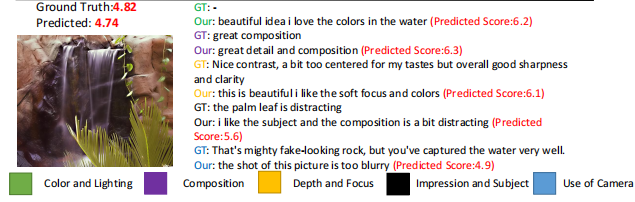
\includegraphics[width=1\textwidth]{11.png}    
 	\caption{The results of aesthetic multi-attribute network on DPC-Captions dataset. The predicted captions and score eachattribute are shown. The Ground Truth score above each image is the global score from DPChallenge.com. The Predicted score above each image is the average score of the 5 predicted scores of attributes.}
 	\label{fig:11}
\end{figure*}


\subsection{Results}
This paper train and test AMAN on the DPC-Captions and PCCD datasets. Some test results on the DPC-Captions dataset are shown. It is worth noting that the results that produce are not
only rich in sentence structure, but also very accurate in grasping features. The relevance of comments and attributes are high. In terms of scoring, average attribute score is very close to the ground truth score. Through the scores and comments, the evaluation of the image is vivid. The captioning and scoring results on PCCD dataset are shown in the supplementary materials due to the page limitation.The results can produce a variety of attribute results.

\section{Conclusion and discussion}
In this survey,we mainly introduce the task of aesthetic attributes assessment of images.Image Aesthetic Quality Assessment (IAQA) is to give an assessment of images on the aspect of aesthetics.The framework to achieve this model is mainly based on the image captioning work.In this survey,we also introduce the development of image captioning work in the last decade.Image captioning work is mainly based the architecture of encoder-to-decoder framework.The introduction of the attention mechanism greatly improves the image captioning work.AMAN is a novel network that can generate captions and scores of each aesthetic attribute.

In the future,it is worthful to achieve captions from sentences to paragraphs.The transfer methods can also be used to build larger dataset for weakly supervised learning.Besides,The relations among attributes can not only be used for scoring learning but also for caption learning.








\bibliographystyle{unsrt}
\bibliography{main}

\end{document}
